\chapter{Weryfikacja rozwiązania}

W celu weryfikacji poprawności działania zaiplementowanego systemu zostały
wykonane serie testów. System został przetestowany pod kątem sprawdzenia
podstawowych założeń projektowych tj. poprawności wykrywania anomali, związanych
z natężeniem ruchu, w obsługiwanej sieci oraz możliwości skalowania
aplikacji \textit{sdn\_epc} w celu zwiększenia wydjaności systemu.
Przeprowadzenie testów wymagało przygotowania odpowiednich scenariuszy testowych,
zestawienia dedykowanych topolgi sieciowych oraz stworzenia rozwiązań
pozwalających na zebranie własciwych danych z testowanego systemu. Analiza
tychże wyników pozwoliła na stwierdzenie, czy i w jakim stopniu założenia
projektowe zostały spełnione. Niniejszy rozdział szczegółowo opisuje
poszczególne przypadki testowe oraz prezentuje analizę uzyskanych wyników.

\section{Test działania implementacji algorytmu}

% w jaki sposób sprawdzamy czy algorytm działa? Liczymy entropie, trzeba to
% ująć
 
Aby stwierdzić, czy zaimplementowany algorytm spełnia swoją rolę tzn. pozwala
wykryć atak DDoS w sieci SDN zostały przeanalizowane wartości entropii obliczone
za pomocą tegoż właśnie algorytmu w dwóch różnych przypadkach testowych, z
których każdy wykorzystywał nieco inną konfigurację testową topologi sieciowej,
jak również samej aplikacji \textit{sdn\_epc}. Przetestowane zostały przypadki, gdy:
\begin{enumerate}
  \item Ruch wygenerowany w sieci testowej był obsługiwany tylko przez jeden
    węzeł aplikacji \textit{sdn\_epc}.
  \item Ruch wygenerowanych w sieci testowej był obsługiwany przez wiele węzłów
    aplikacji \textit{sdn\_epc} działających w klastrze.
\end{enumerate}
Wykorzystanie takich właśnie przypadków testowych umożliwiło sprawdzenie
poprawności implementacji algorytmu zarówno w przypadku działania systemu jako
pojedynczy węzeł aplikacji \textit{sdn\_epc}, jak również w przypadku, gdy
system działał w klastrze. Drugi przypadek jest znacznie bardziej złożony,
ponieważ rozproszenie procesu obliczania algorytmu na wiele węzłów wprowadza
dodatkowe komplikacje, związane z synchronizacją stanu pomiędzy węzłami w
klastrze.

\subsection{Przypadek testowy z wykorzystaniem jednego węzła aplikacji
  \textit{sdn\_epc}}

Schemat topologii sieciowej, wykorzystanej w przypadku, gdy tylko jeden węzeł
aplikacji jest zaangażowany w przetwarzenie ruchu został przedstawiony na
Rys. \ref{fig:entropia_scheme}.

\begin{figure}[h]
\centering
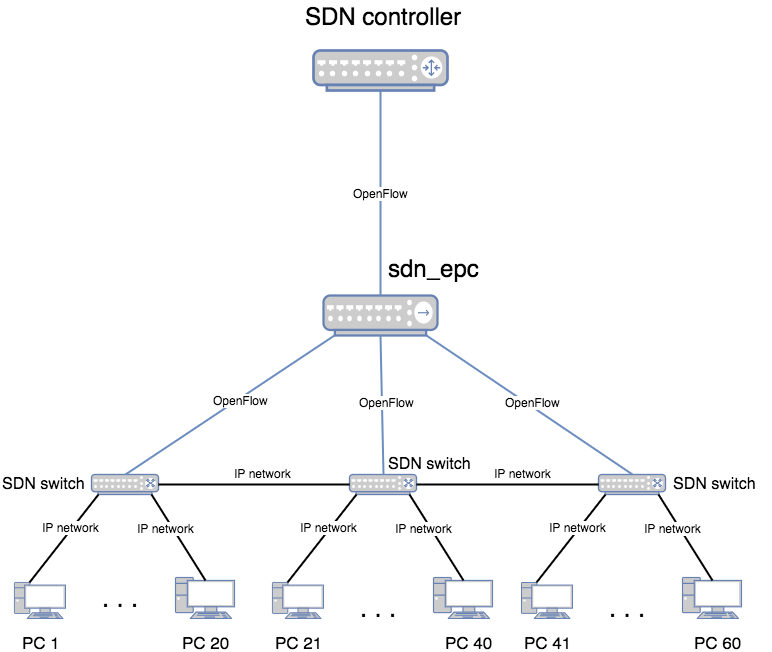
\includegraphics[width=\textwidth]{entropia_scheme}
\caption{Schemat topologii sieciowej z wykorzystaniem jednego węzła aplikacji
  \textit{sdn\_epc}.}
\label{fig:entropia_scheme}
\end{figure}

W topologii przedstawionej na Rys. \ref{fig:entropia_scheme} wszystkie
przełączniki obsługujące ruch pomiędzy węzłami końcowymi (\textit{PC N})
komunikują się z kontrolerem (\textit{SDN controller}) poprzez jeden węzeł
aplikacji \textit{sdn\_epc}. Wykorzystując taką konfigurację sieci, tylko jeden
węzeł \textit{sdn\_epc} przetwarza wiadomości \mbox{\textit{PACKET\_IN}}
protokołu \textit{OpenFlow}, wymieniane pomiędzy poszczególnymi przełącznikami,
a kontrolerem, w celu obliczenia entropii pakietów przesyłanych w sieci.

Jeśli algorytm został poprawnie zaimplementowany to wartość entropii,
obliczonej za jego pomocą, powinna maleć wzraz ze spadkiem losowości pakietów
przesyłanych w sieci testowej. Innymi słowy, im więcej pakietów w sieci jest
adresowanych do pojedynczego węzła końcowego, tym mniejsza będzie wartość
obliczonej entropii.

W celu sprawdzenia czy wspomiana zależność została spełniona, koniecznym było
zaprojektowanie odpowiedniego scenariusza testowego. Scenariusz ten opierał się
na środowisku testowym przedstawionym na Rys. \ref{fig:entropia_tech}.

\begin{figure}[h]
\centering
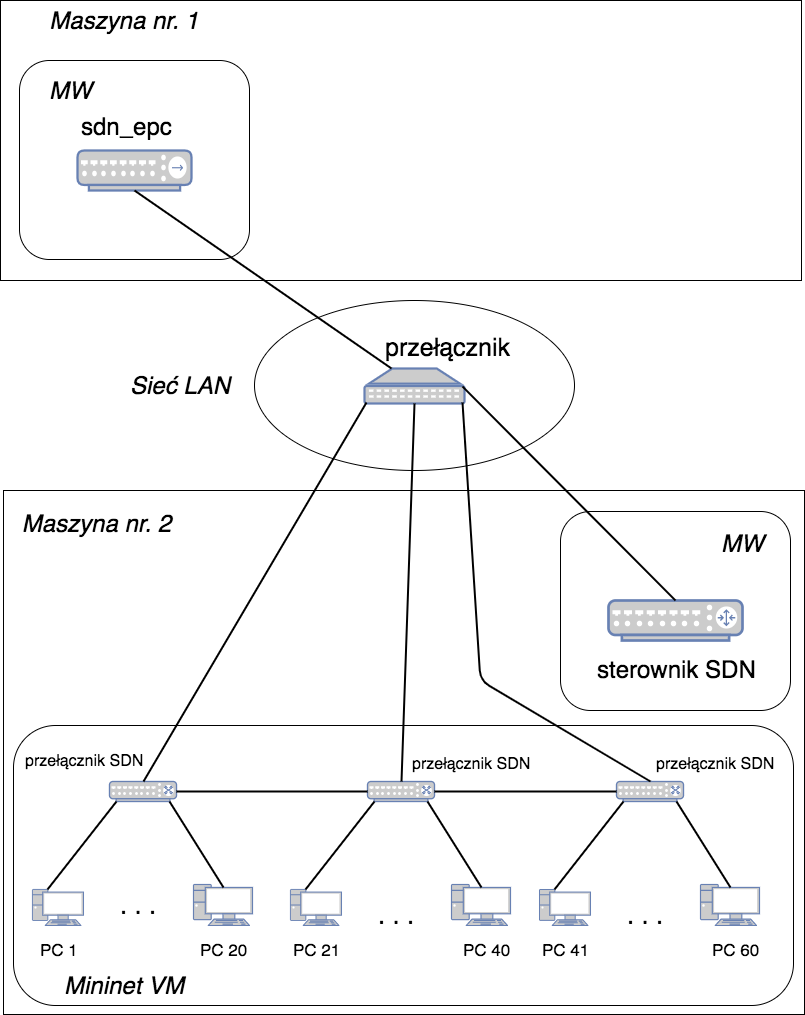
\includegraphics[height=11cm]{entropia_tech}
\caption{Środowisko testowe z wykorzystaniem jednego węzła aplikacji
  \textit{sdn\_epc}.}
\label{fig:entropia_tech}
\end{figure}

Jak przedstawiono na Rys. \ref{fig:entropia_tech} toplogia sieciowa została
zestawiona z użyciem dwóch maszyn fizycznych, na których zostały zwirtualizowane
niezbędne komponenty testowe. Każdy z komponentów, za wyjątkiem przełącznika
sieci \textit{LAN} (\textit{switch}), został uruchomiony na dedykowanej maszynie
wirtualnej. Jako środowisko do wirtualizacji zostało wykorzystane oprogramowanie
\textit{VirtualBox \footnote{https://www.virtualbox.org}}. Maszyny wirtualne
komunikowały się ze sobą z wykorzystaniem sieci \textit{LAN}.

Przełączniki sieci SDN (\textit{SDN switch}'es) oraz węzły końcowe (\textit{PC
  N}) były emulowane na dedykowanej maszynie wirtualnej za pomocą oprogramowania
\textit{Mininet \footnote{http://mininet.org}}. Wykorzystane w teście
przełączniki to domyślne przełączniki używane przez oprogramowanie
\textit{Mininet}, które działają na bazie oprogramowania
\textit{Open vSwitch \footnote{http://openvswitch.org}}.
\textit{SDN controller}, pełniący funkcję kontrolera w testowej topologii,
korzystał z oprogramowania zbudowanego z wykrzystaniem framework'a
\textit{Ryu \footnote{https://osrg.github.io/ryu}}. Maszyny wirtualne dedykowane
dla \textit{sdn\_epc} i \textit{SDN controller} działały pod kontrolą systemu
operacyjnego \textit{Ubuntu \footnote{https://www.ubuntu.com}}.

Scenariusz testowy zakładał przeprowadzenie kilku prób, podczas których w sieci
były generowane ataki DDoS o różnej sile. Podczas każdej próby została zmierzona
średnia wartość entropii obliczonej za pomocą zaimplementowanego algorytmu.
Wykonane zostały cztery próby z atakami o sile odpowiednio: 0\%, 30\%, 60\% oraz
90\%. Siła każdego ataku została obliczona na podstawie wzoru
\ref{equ:ddos_power}

\begin{equation}
\label{equ:ddos_power}
R = \frac{P_{a}}{P_{n}} \cdot 100\%
\end{equation}
gdzie R oznacza siłę ataku, $P_{a}$ pakiety atakujące, natomiast $P_{n}$ pakiety
tła.

Pakiety tła rozumiane są jako pakiety
\textit{IP \footnote{https://tools.ietf.org/html/rfc791\#section-3.1}} wysyłane
do losowo wybranych węzłów końcowych w stałych odstępach czasowych. Pakiety
atakujące oznaczają pakiety \textit{IP}, które zawierają losowe adresy docelowe
oraz są wysyłane do konkretnego węzła końcowego w 4-krotnie krótszych odstępach
czasowych. 